\subsection{Mô hình dữ liệu đề xuất}\label{sec:system-data-models}
CDM (Hình~\ref{fig:database-cdm}), LDM (Hình~\ref{fig:database-ldm}) và PDM (Hình~\ref{fig:database-pdm}) mô tả thiết kế tích hợp đầy đủ. CDM xác định thực thể nghiệp vụ; LDM bổ sung lần chạy, cụm và họ bằng chứng; PDM cụ thể hóa khóa, kiểu dữ liệu và ràng buộc SQLite. Các bảng phân tích bổ sung thuộc thiết kế đề xuất; phiên bản hiện tại dùng bảy bảng nêu trên và cache kết quả cụm trong bộ nhớ.

\begin{reportlandscapefigure}
\centering

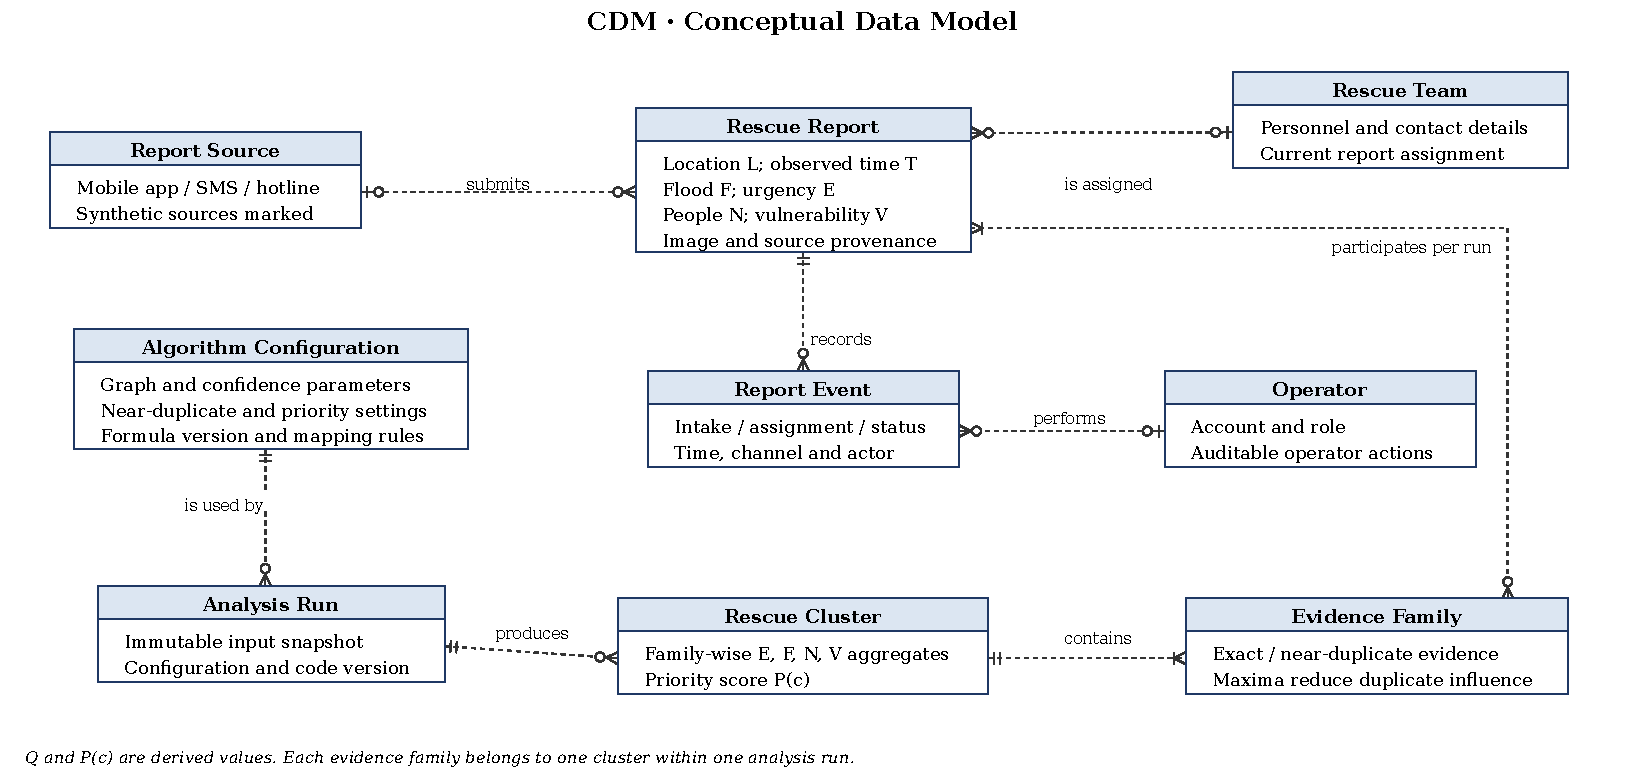
\includegraphics[width=\linewidth,height=\ReportLandscapeImageHeight,keepaspectratio]{diagram-revisions/2026-10-29-data-models-review/01-cdm.pdf}
\caption{Mô hình dữ liệu khái niệm (CDM) của hệ thống cứu hộ}
\label{fig:database-cdm}
\end{reportlandscapefigure}

\begin{reportlandscapefigure}
\centering

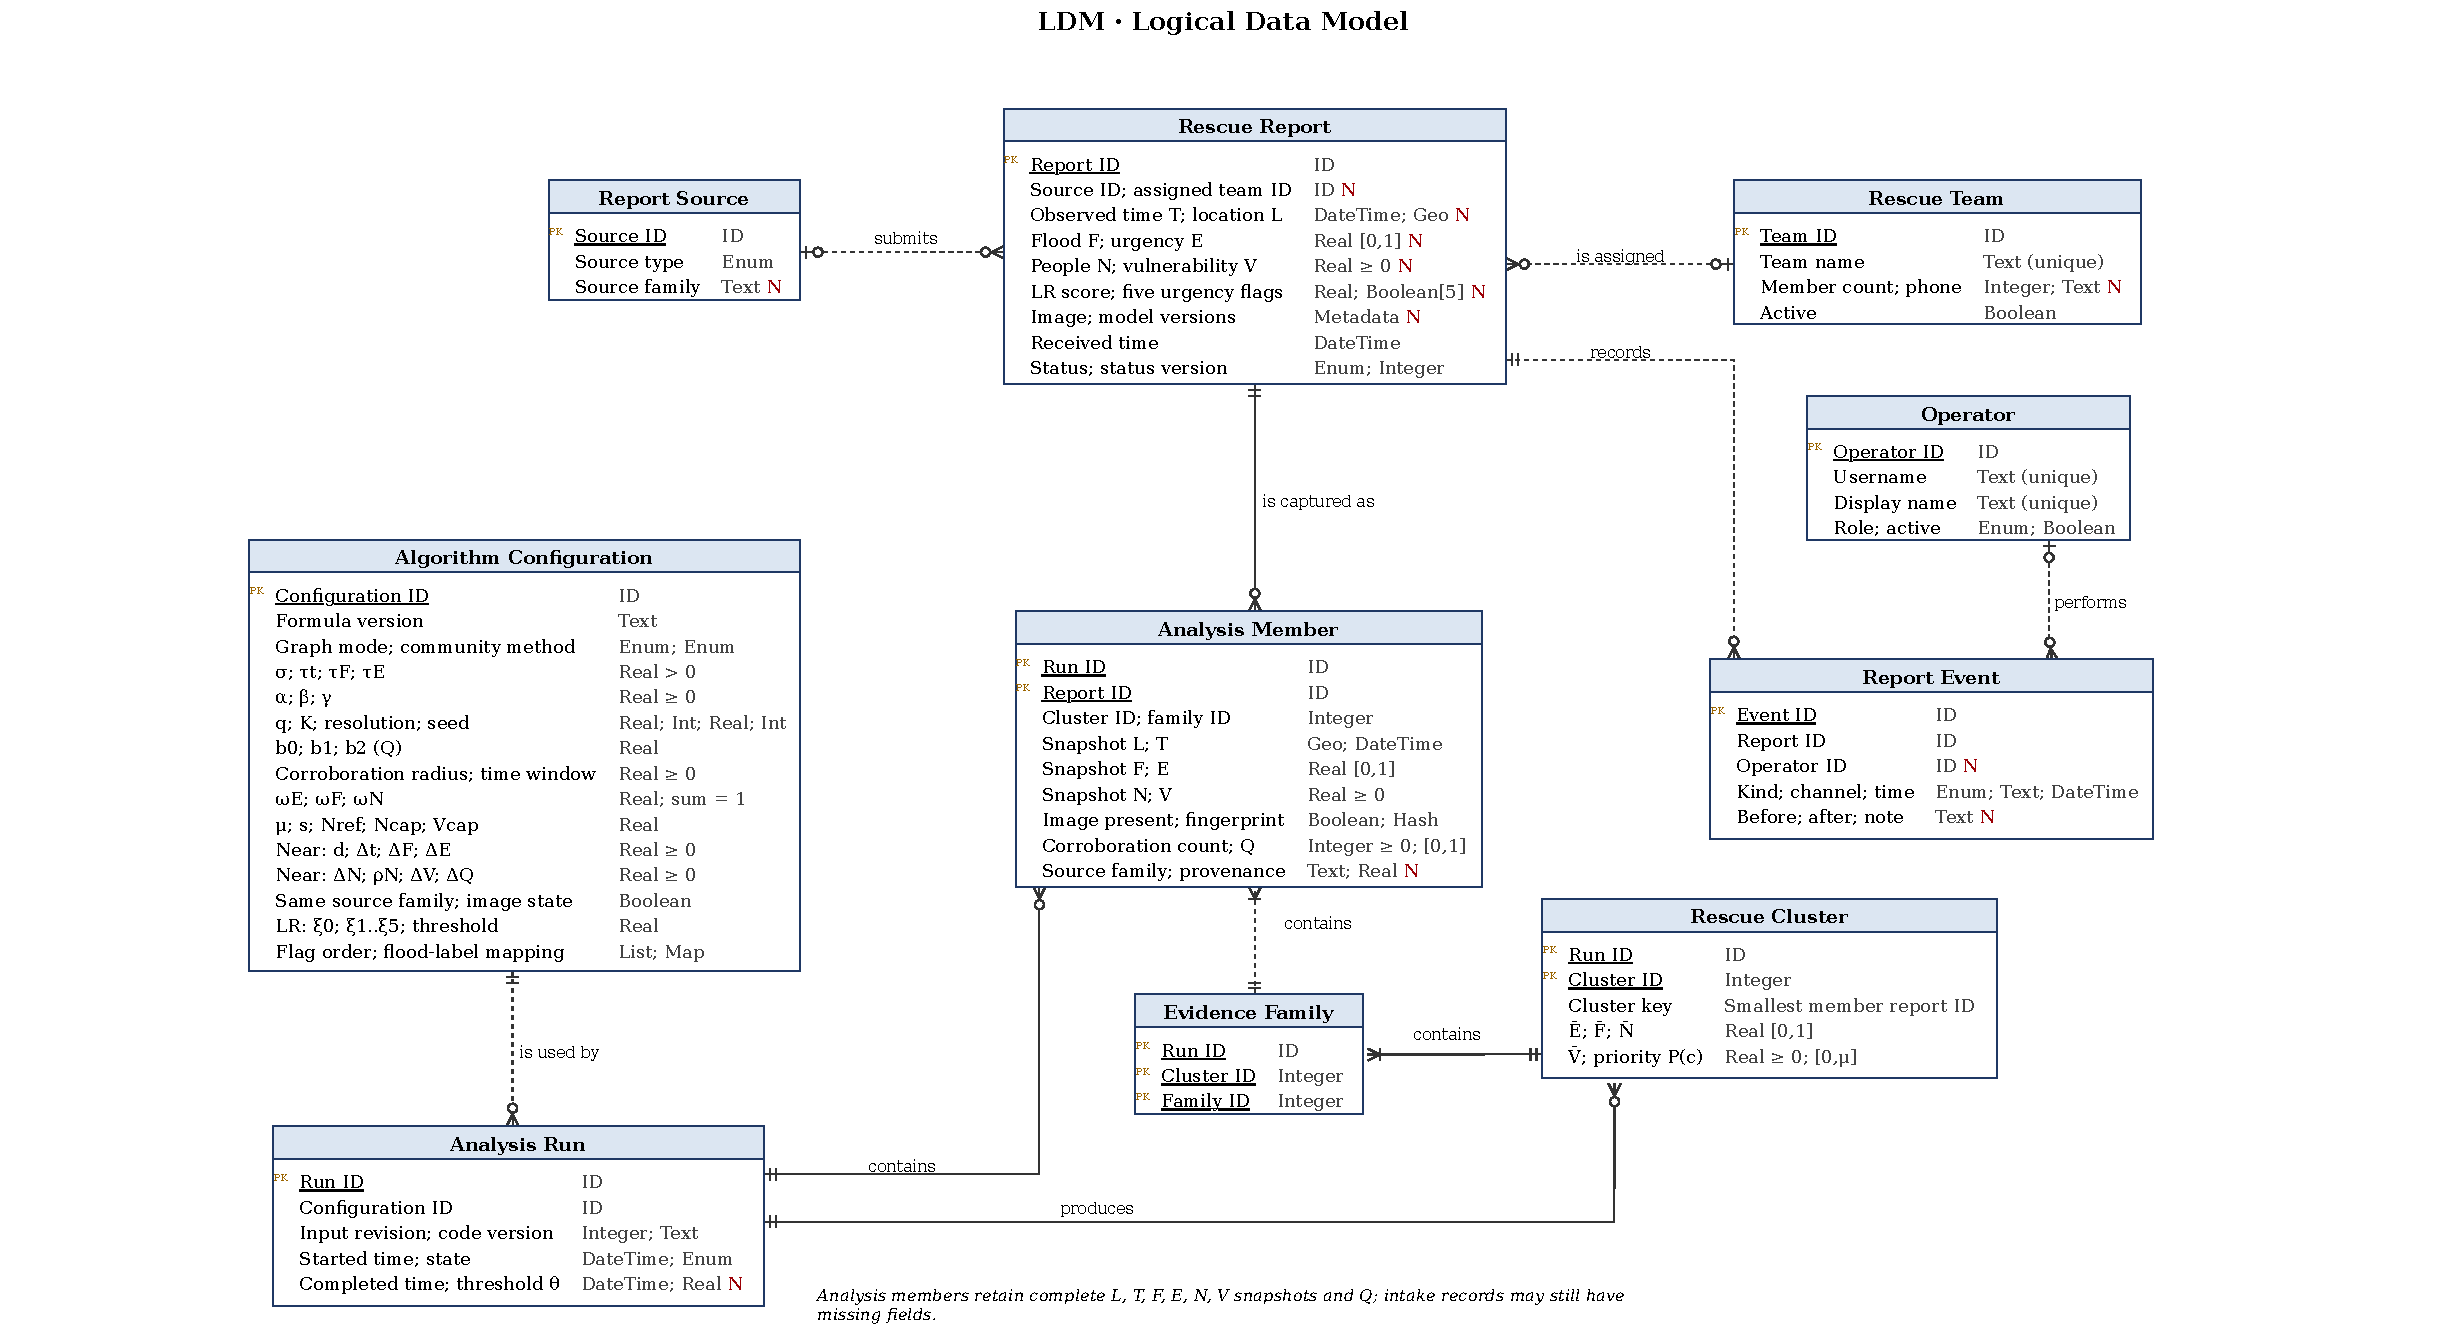
\includegraphics[width=\linewidth,height=\ReportLandscapeImageHeight,keepaspectratio]{diagram-revisions/2026-10-29-data-models-review/02-ldm.pdf}
\caption{Mô hình dữ liệu logic (LDM), định danh và cấu hình phân tích}
\label{fig:database-ldm}
\end{reportlandscapefigure}

\begin{reportlandscapefigure}
\centering

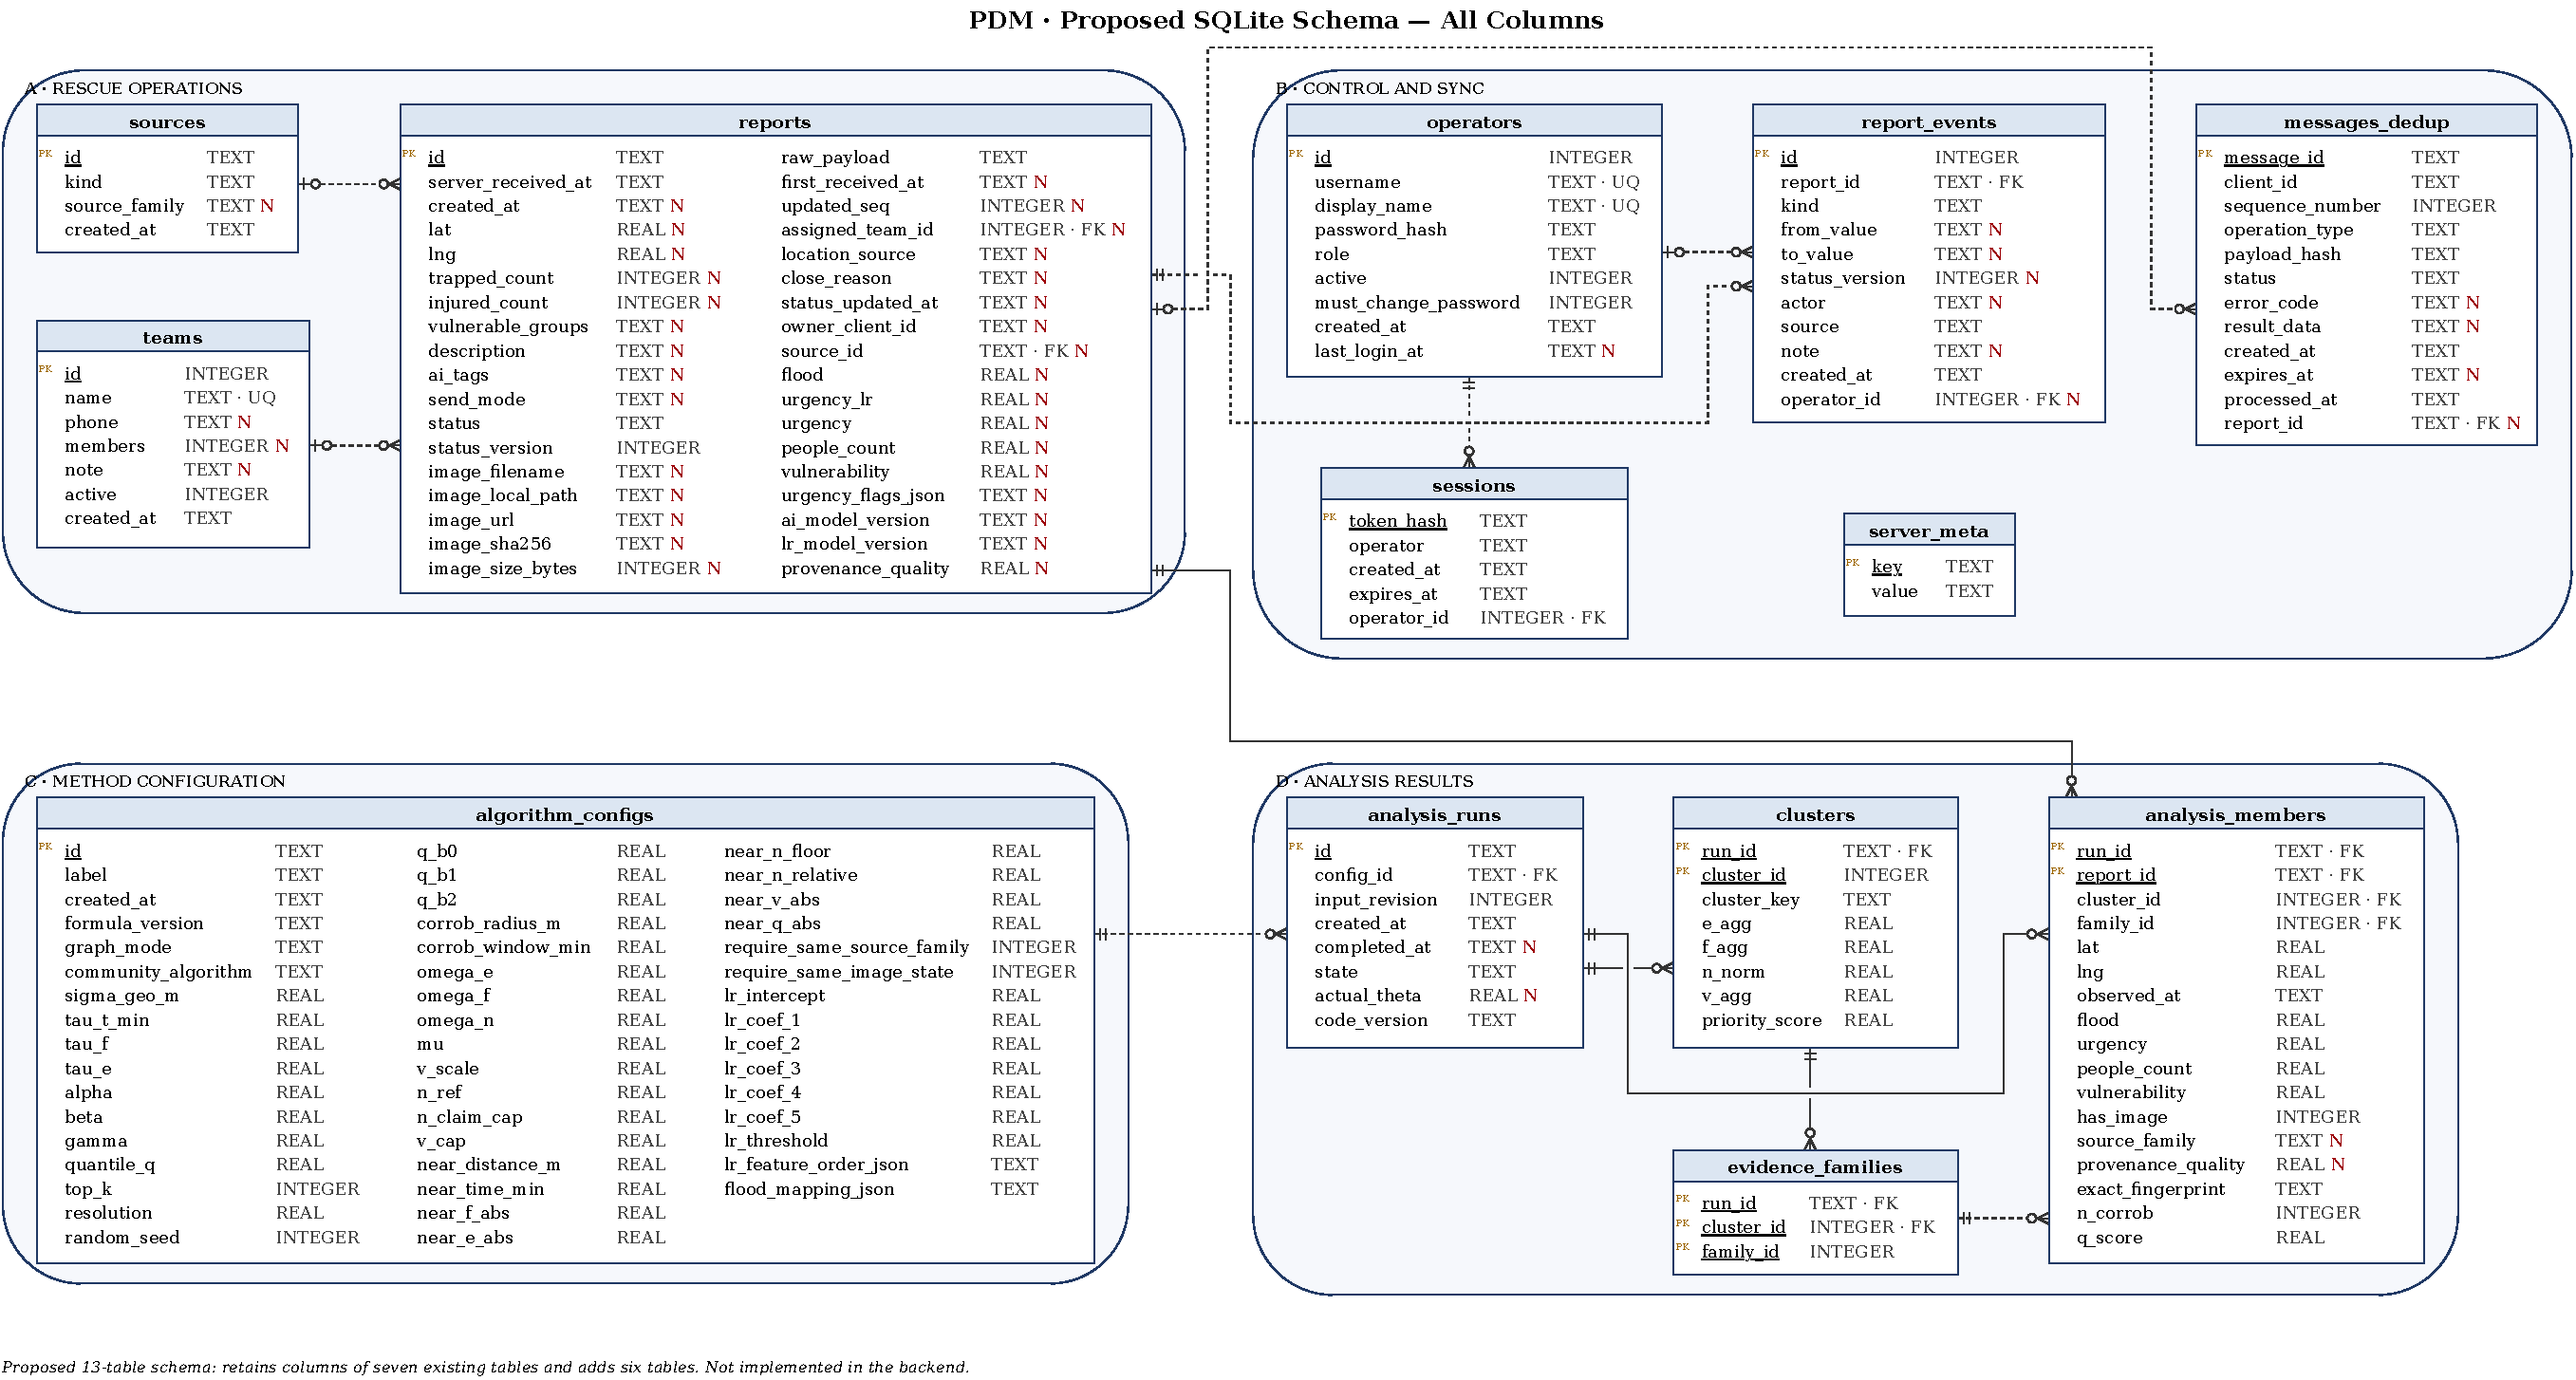
\includegraphics[width=\linewidth,height=\ReportLandscapeImageHeight,keepaspectratio]{diagram-revisions/2026-10-29-data-models-review/03-pdm.pdf}
\caption{Mô hình dữ liệu vật lý (PDM) đề xuất trên SQLite}
\label{fig:database-pdm}
\end{reportlandscapefigure}

\FloatBarrier
